

\section{Storytelling} 
%\label{sec:}
Parallelen zwischen Film und Videospielen, bewegtes Bild und Ton

Aber Spiele funktionieren anders

Filme bieten keine interaktivität oder auswahlmöglichkeiten, sind keine präsenz(zeit) erfahrung

Museen und Kunstgalerien sind interaktiv nichtlinear bei denen der besucher zwar in eine richtung gelenkt wird aber sie dennnoch auf seine eigene art durchläuft. bei ruinen und grafties ist das ähnlich. 
aber auch der tatort eines verbrechens kann als eine interaktive erzählung sein. so muss der ermittelnde polizist aus den einzelnen details wie blutspuren und zerbrochenem glas schließen, was vorgefallen ist.


die meisen medien haben nur wenig werkzeuge.
comicbuch hat sprechblasen und bilder, ein kinofilm hat 24 fps und verschiedene audiospuren. ein romanautor eine bestimmte anzahl an worten. ein aussteller in einem museum erhält seinen zugewiesenen platz mit dem zugehörigen layout, info panäle und evtl ein diorama und oder ein paar interaktive spielereinen.

spiele decken einen größeren Bereich ab. sie bieten die Fähigkeiten von bewegten Bildern und sounds, können zudem aber noch Texte wie in einem buch oder in einer Sprechblase, wie in einem comic, wiedergeben. der Nutzer hat dabei sogar die Möglichkeit ganze Kapitel oder Seiten zu überspringen. es können aber auch wie im museum bereiche definiert werden, an denen der spieler die geschichte selbst erkundet. hinzu kommen weitere Werkzeuge, die im keinen der zuvor genannten Medien vorhanden sind. So können Spiele durch die Spielmechaniken die sowohl die handlung des spiels beeinflussen, die charakterentwicklung, aber auch die Szenerie augenblicklich ändern können. wobei diese anderen mit den Entscheidungen des spielers verknüpft sind.
dies zeigt, wie stark die Erzählweise in spielen von den herkömmlichen abweicht.
so lässt sich an dieser stelle die Erzählweisen in drei Bereiche zusammenfassen. der scripted story, also der zu vor festgesetzten Geschichte, der World narrative, der Geschichte die eine Szene von sich erzählt und der exklusiv den Videospielen zugehörigen emergent story, eine Geschichte, die zur Laufzeit des Spieles entsteht.

die simpelste Variante der scripted story ist die cutscene, zu deutsch, zwischensequenz. Mit ihr stehen dem Entwickler/storywriter alle tricks des films, wie emotionale closeups zur Verfügung. Diese bringen aber immer einen harten Übergang mit sich, denn dem Spieler wird die Kontrolle über das Spiel entzogen. Werden Cutscenes zu häufig eingesetzt, wird der Ablauf des Spiels zu einem stop-start Erlebnis und somit abgehackt wirken. Richtig eingesetzt, können sie aber eine gute Trennung von Spielabschnitten darstellen. Trotzdem sind die cutscenes immer ein holpriger Übergang. 

Um den Übergang zwischen einer Cutszene und dem Hauptspiel fließender zu machen, gibt es den sog. soft-scripted Ansatz. Bei diesem Ansatz wird dem Spieler weiterhin die Kontrolle überlassen. Er kann also z.b. seinen Charakter weiter steuern. Hierdurch verliert aber der Designer einen Großteil der Kontrolle über die Szene. Dies bringt den Nachteil mit sich, das der Spieler die jeweilige Szene aus einem ungünstigen Blickwinkel oder ggf. gar nicht sehen kann. Es wäre auch denkbar, dass der Spieler versucht eine Interaktion durchzuführen, die nicht vorgesehen ist, wie eine für die story wichtige Person zu erschießen. 

%
%The advantage of this soft-scripted approach is that it doesn’t break flow since the player’s controls remain uninterrupted. The downside is the control it takes away from the designer. The player might be able to watch the murder from an ugly angle, miss it entirely, or even interfere with it.
%For example, a hint might require enemies to stay in the rear half of a room, but still allow them to autonomously shoot, grab cover, dodge grenades, and punch players who get too close. Designers use these hints to author higher-level strategic movements, while the AI handles moment-by-moment tactical responses to player behavior.
%
%There are also ways of scripting events which are naturally immune to interference. Mail can arrive in the player character’s mailbox at a certain time. Objects or characters can appear or disappear while the player is in another room. Radio messages and loudspeaker broadcasts can play. These methods are popular because they are powerful, cheap, and don’t require the careful bespoke design of a custom semi-interactive scripted sequence.
%
%All places tell stories. We can explore any space and discover its people and its history. Game designers can use this to tell a story by embedding it in a space. I call this world narrative.
%
%Next, world narrative does not need to be told in linear order. This saves us from having to railroad players into a specific path. For example, imagine that the narrative content is that two lovers fought, and one mur- dered the other and buried him in the backyard. Told through the world narrative a day later, it doesn’t matter if the player discovers the corpse or the bloody bedroom first. As long as he sees both, in either order, he will be able to piece together what happened. This means that a game de- signer can let the player explore the house freely. Telling the same story in scripted events would require that the designer come up with some trick or restriction to ensure players follow the right path through the space in order to see all the events in the right order.
%
%
%World narrative’s last great advantage is that it supports players re- playing the game because it doesn’t always reveal itself completely the first time around. Whereas scripted stories uncover themselves event by event from start to finish, world narrative naturally uncovers itself in order
%
%
%When you play a racing game against a friend and come back to win after a bad crash, that’s a story. But it wasn’t written by the game de- signer—it emerged during your particular play session. This is emergent story.
%We can look at emergent story in two ways: as a narrative tool, and as a technology for generating story content.
%
%Showing and telling players less creates more room for apophenia to fill in the gaps.
%
%More detailed graphics and higher-quality sound add something to a game, but they also take something away. The more detailed the graphics, sound, and dialogue of a game, the less space there is for interpretation.The more abstract, nonspecific, and minimalistic the representation, the more apophenia becomes possible.
%
%
%
%But most narrative tools still work better when we control the order in which they’re used. Sometimes we want to ensure the setup occurs before the payoff. We might want to let one subplot play out before we add another so we don’t have too many plot threads running at once.
%
%
%
%Or perhaps we want to introduce game mechanics one by one alongside the story so we can train the player in a smooth progression. In each case, we need some way to make sure one piece of content is consumed before another.
%
%
%Quests    blockage     Skill gating 
%
%...
\section{Erzählstrukturen in Videospielen} 
%\label{sec:}
 

\subsection{Lineare Struktur} 
%\label{sec:}

Diese Erzählweise spiegelt ein Buch oder einen Film wieder. Übertragen auf ein Spiel heißt das, dass der Spieler mit jedem Level einen Schritt weiter durch die Story geführt wird. Hierbei ist jedoch zu beachten, wie der Umfang der Storyelemente gewählt wird. Das Spielen von kleinen Levels mit wenig Geschichte kann schnell dazu frühen, dass das der Spieler sich stark in seinem Handlungsrahmen eingeschränkt fühlt.  Dieses Erzählweise wurde z.B. in den klassischen Super Mario Bros. Spielen aber auch in etlichen anderen Spielen, wie z.B Quake oder dem Singleplayer von Stracraft, verwendet.


\begin{figure}[H]
    \centering
    
\includegraphics[width=.8\textwidth]{files/story/storyLinear}
    \caption{Veranschaulichung der linearen Struktur}
    %\label{szenA}
\end{figure}
 
\subsection{Zentraler Knotenpunkt} 
%\label{sec:}
Bei dem zentralen Knotenpunkt handelt es sich um ein Level, mit dem alle anderen Level verbunden sind. Dem Spieler steht somit ein zentrales Level zur Verfügung, von dem aus er die Geschichten der anderen Level in beliebiger Reihenfolge erleben kann. Es kann auch in erweiterter Form auftreten, bei der ein Spieler erst einige Level gespielt haben muss, um weitere Level freizuschalten. So kann der Spieler in einem gewissen Maß selber festlegen, wie die Story voranschreitet. 
Die basis Version hiervon ist in den Megaman Spielen zu finden. Dort kann der Spieler in einer Art Menü auswählen, welches Level er als nächstes spielen möchte. In Super Mario 64 ist eine erweiterte Version dieses Modells realisiert. Der Spieler bewegt sich in einem Schloss und hat auch die Möglichkeit verschiedene Level zu starten. Es ist ihm aber nicht möglich von Anfang alle Level zu betreten ua. auch weil einige Level versteckt sind und nur durch Zufall vom Spieler entdeckt werden können. Des Weiteren müssen nicht alle Level gespielt werden, um die Hauptgeschichte des Spiels abzuschließen.


\begin{figure}[H]
    \centering
    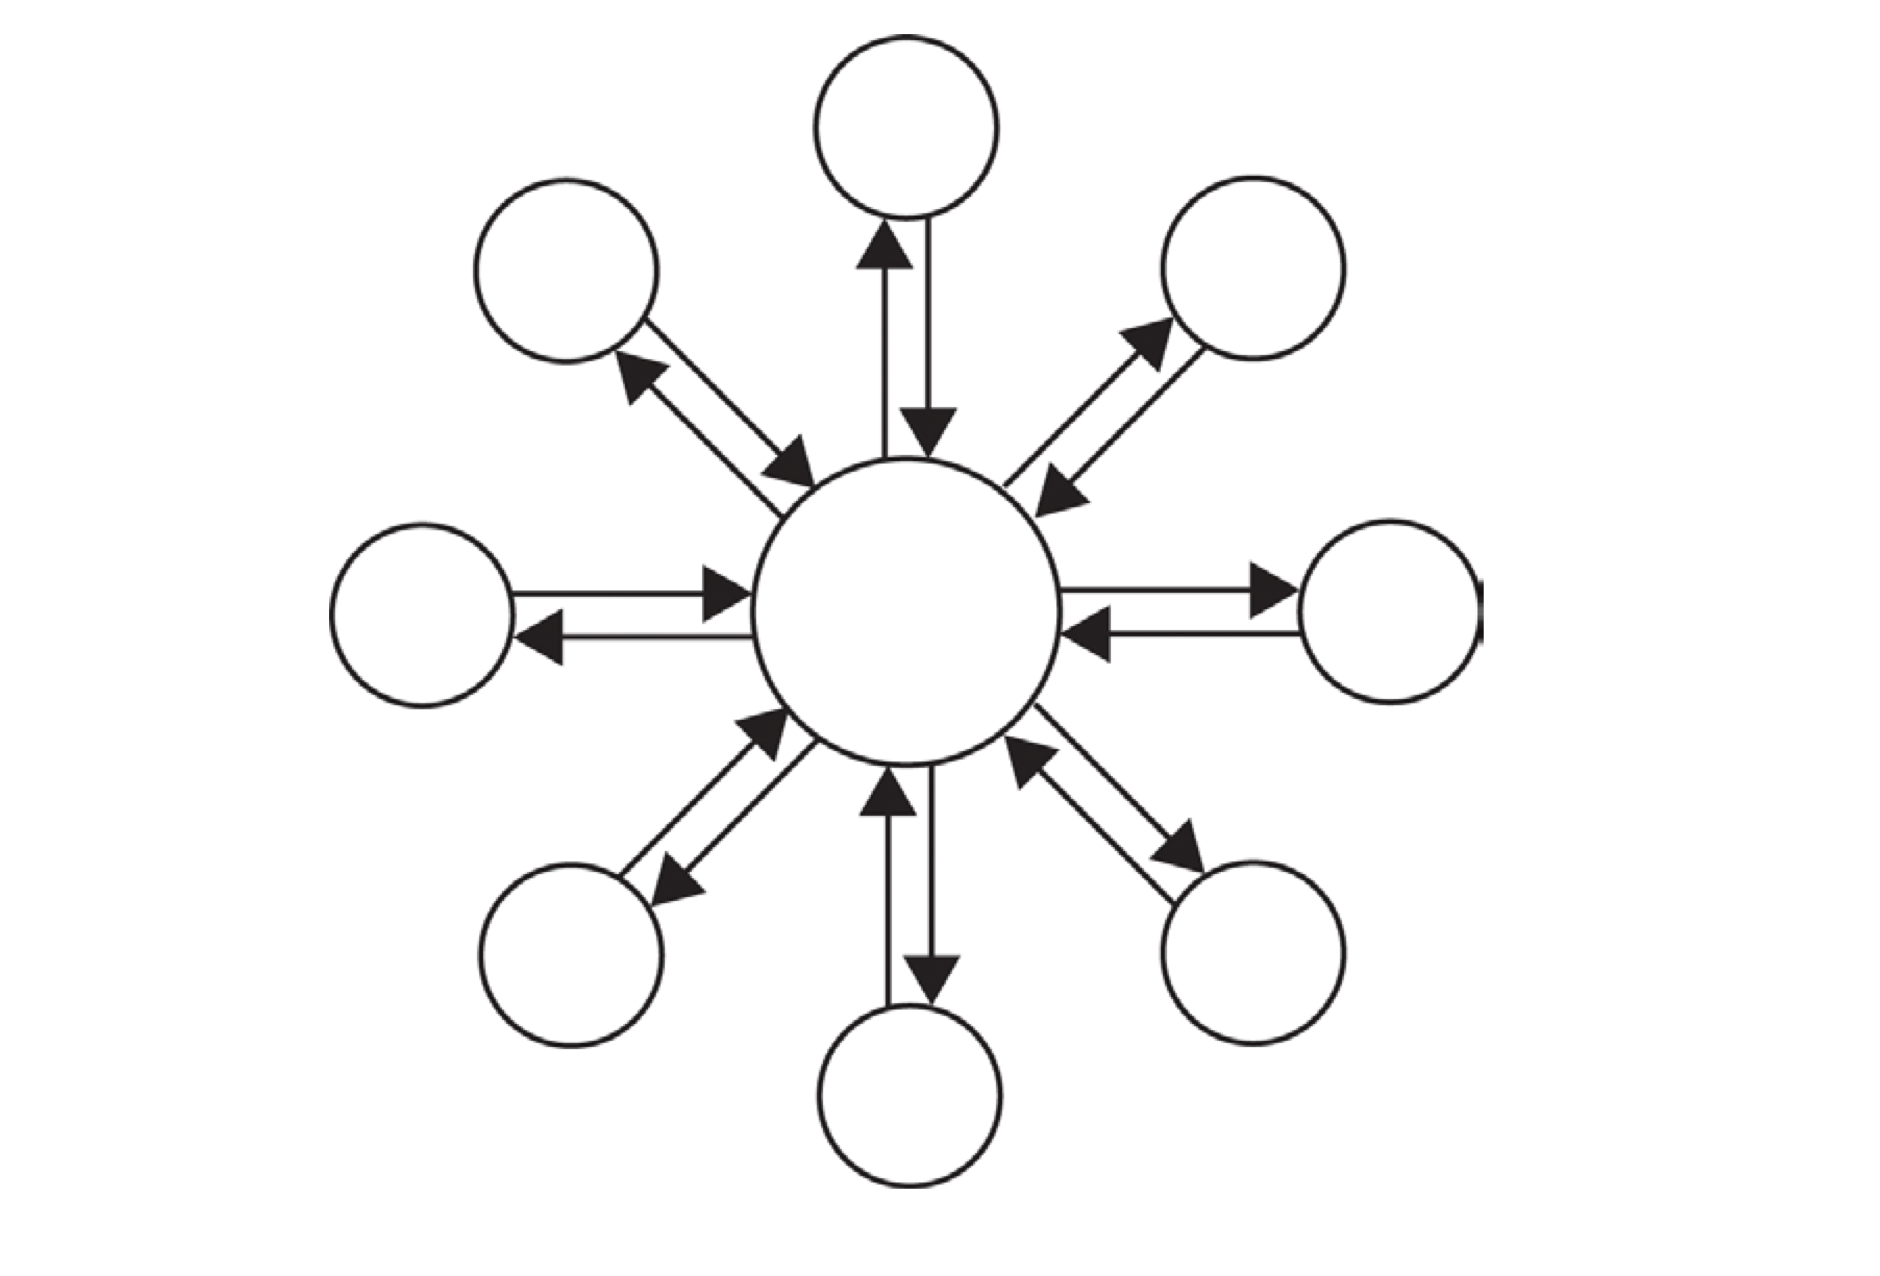
\includegraphics[width=.8\textwidth]{files/story/storyZentralKnoten}
    \caption{Veranschaulichung des zentralen Knotenpunkt}
    %\label{szenA}
\end{figure}


 
\subsection{Komplett Entscheidungsgesteuert} 
%\label{sec:}

An des reale Leben angelehnt.
Exponentieller Wachstum. 
Spielern wird viel vorenthalten. 
 
\begin{figure}[H]
    \centering
    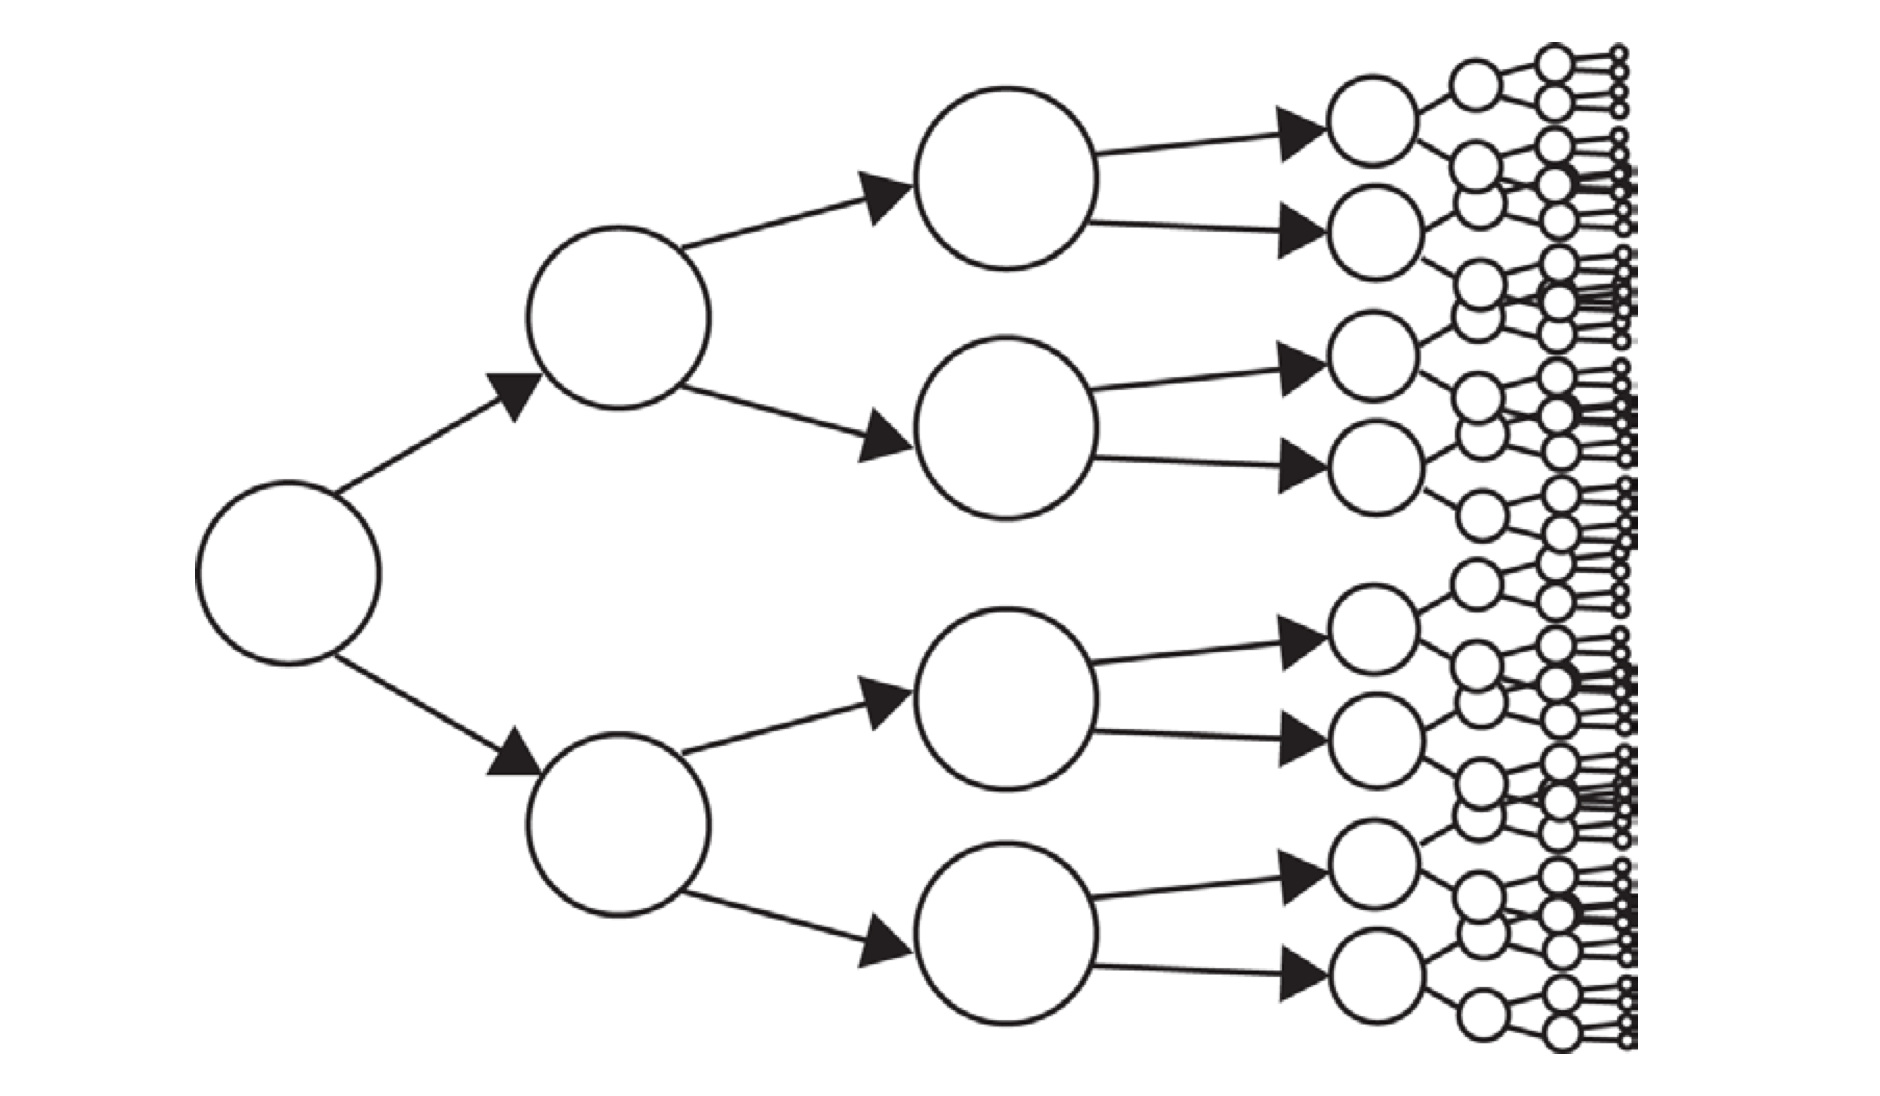
\includegraphics[width=.8\textwidth]{files/story/storyEntscheidungen}
    \caption{Veranschaulichung der komplett Entscheidungsgesteuerten Variante}
    %\label{szenA}
\end{figure} 
 

\subsection{Nicht lineare Story mit optionalen Sidequests} 
%\label{sec:}

Es ist möglich nicht die ganze Story zu erleben
Ein Teil der Story ist abgekapselt
Haupstory verläuft zum Linear, kleine Exkursion

\begin{figure}[H]
    \centering
    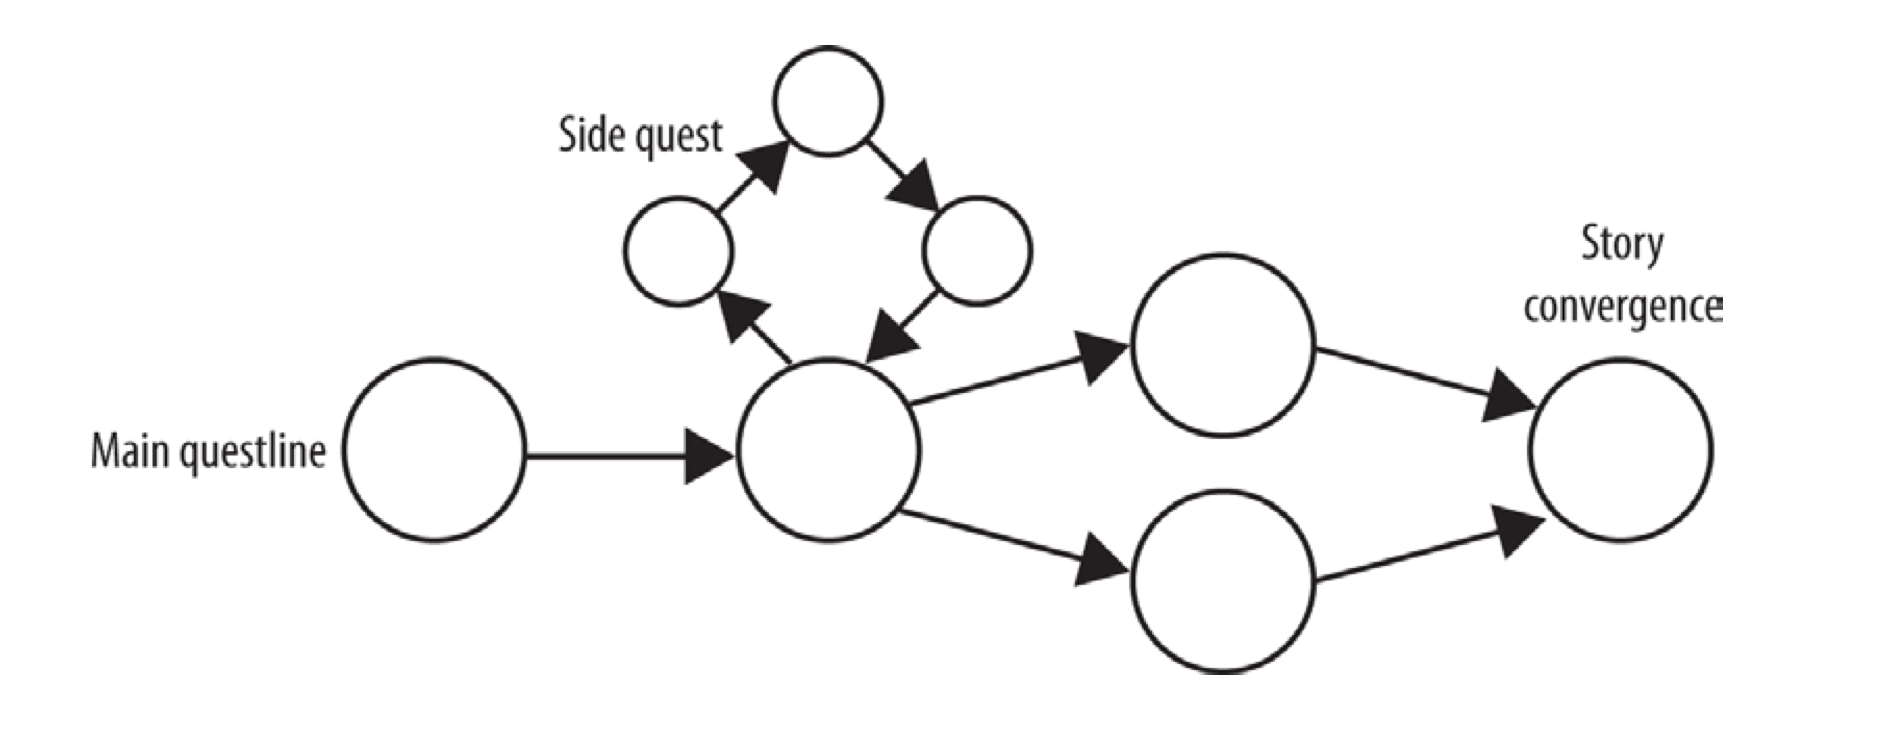
\includegraphics[width=.8\textwidth]{files/story/storySidequest}
    \caption{Veranschaulichung der nicht linearen Story mit Sidequest}
    %\label{szenA}
\end{figure} 
 
\subsection{Zentraler Knotenpunkt mit linearem Fortsatz} 
%\label{sec:}

Ähnlich wie oben, aber nachdem die ersten Storyteile gespielt wurden
Wird linear fortgesetzt


\begin{figure}[H]
    \centering
    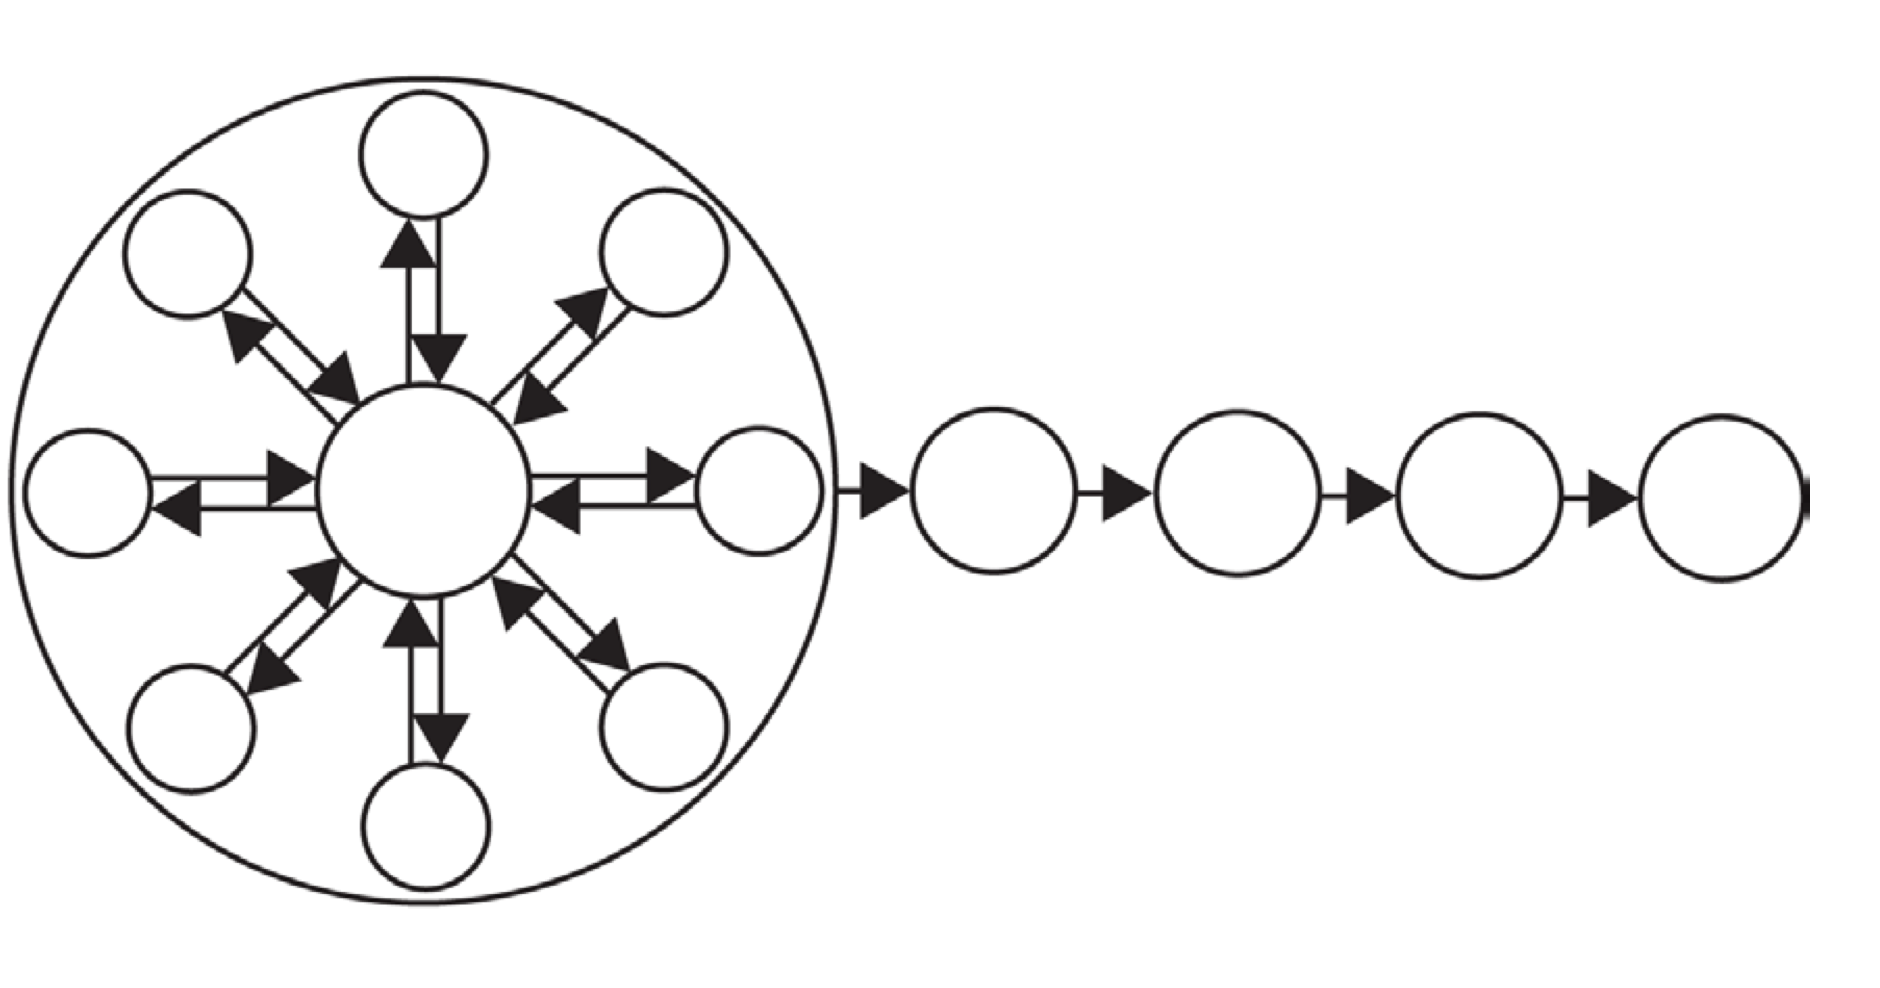
\includegraphics[width=.8\textwidth]{files/story/storyZentralKnotenLinear}
    \caption{Veranschaulichung des zentralen Knotenpunkts mit linearem Fortsatz}
    %\label{szenA}
\end{figure} 


\subsection{Hybrid, Linear und Storyabschnitte} 
%\label{sec:}

Linear mit teilweise verketteten Storytelementen
Anfang und Ende sind linear
Flickenmuster aus Sidequests, die zur hauptgeschichte beitragen
Spieler kann entscheiden, was er erleben möchte.
Kann die Geschichte auch beenden ohne alle Informationen gesammelt zu haben. \\

\begin{figure}[H]
    \centering
    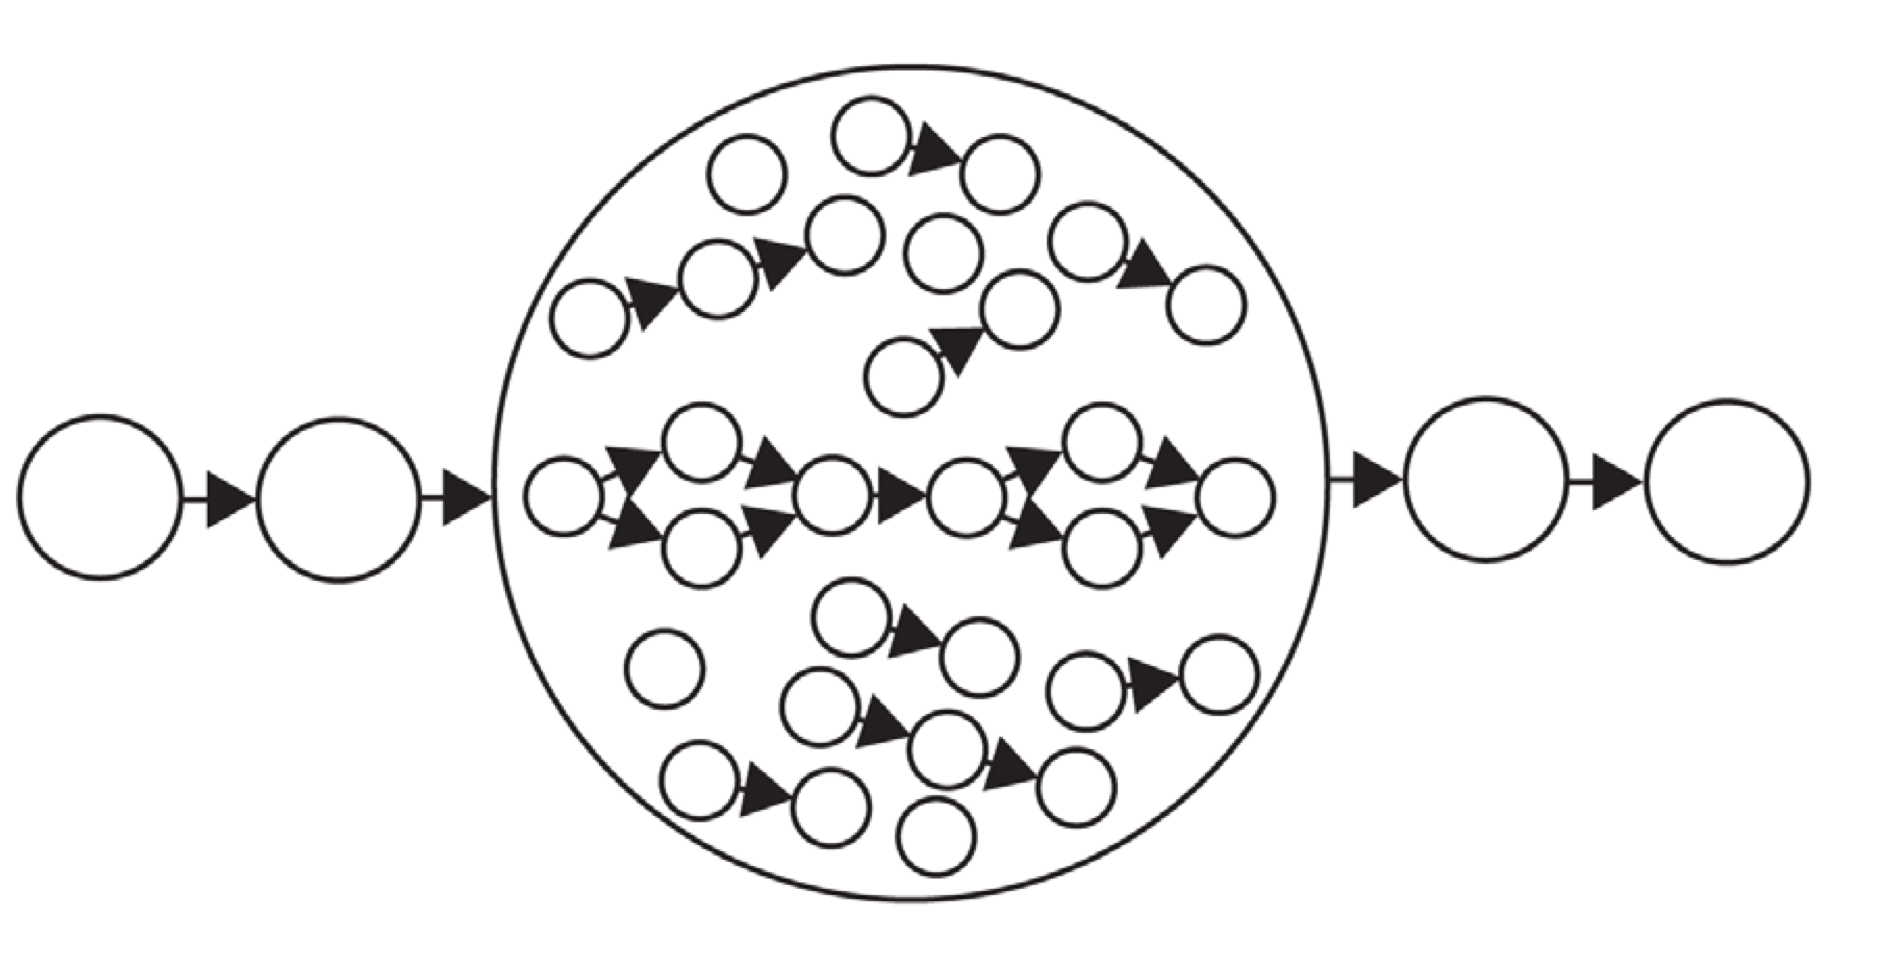
\includegraphics[width=.8\textwidth]{files/story/storyTeile}
    \caption{Veranschaulichung des hybriden Ansatzes}
    %\label{szenA}
\end{figure} 


\cite[Seite 12]{Adams:1515529}